\documentclass[a4paper, british]{article}

\usepackage[utf8]{inputenc}
\usepackage[T1]{fontenc}
\usepackage{babel}
% \usepackage[margin=2.5cm,a4paper]{geometry}
% \usepackage[skip=1em]{parskip}
\usepackage{lmodern} 
\usepackage{microtype}
% \usepackage{xcolor}
\usepackage{graphicx}
\graphicspath{ {./figures/} }
% \usepackage{float}
% \usepackage{enumitem}
\usepackage{adjustbox} % rescale - useful for Dia exported TeX
\usepackage{tikz}
% \usepackage{pgfplots}
\usepackage{booktabs} %tables no vertical lines
% \usepackage{array}
% \usepackage{authblk}
% \usepackage{fancyhdr} %headers and footers
% \usepackage{titlesec}
% \usepackage{tcolorbox} % framed text boxes
% \usepackage{mathtools, amssymb, amsthm}
% \usepackage{gensymb}
\usepackage{chemformula} % chemical formulae
\usepackage{chemfig} % molecular figures
\usepackage{siunitx}
\usepackage{csquotes}
\usepackage[titletoc, title]{appendix}
% \usepackage{lettrine} % initials

\usepackage[
pdfauthor={Adam Menne},
pdftitle={Chemistry 254 - Practical 1},
pdfsubject={},
pdfkeywords={}]{hyperref}

\usepackage[noabbrev]{cleveref}

\usepackage[
backend=biber,
style=numeric,
sorting=none,
doi=true,
isbn=false
]{biblatex}
\addbibresource{citations.bib}

\setlength{\parskip}{1em}
\setlength{\parindent}{0em}
\linespread{1.3}

\title{Chemistry 254\\ Experiment 3\\ Mean activity coefficient of an electrolyte}
\date{Last editted on \today}
\author{Adam Menne\\ Stellenbosch University}

\begin{document}

\maketitle

\begin{abstract}
\noindent
In this practical the effect of electrolyte concentration of th mean activity coefficient was investigated through Debye-H{\"u}ckel theory.
\end{abstract}

\tableofcontents

\newpage

\section{Introduction}
In this practical the effect of electrolyte concentration of th mean activity coefficient was investigated through Debye-H{\"u}ckel theory.

by virtue of the fact that \(log(s) = log(s_0) + Kz_+ z_- \sqrt{I}\), we know that when \(\sqrt{I} = 0\), \(log(s) = log(s_0)\). Thus we can find \(s_0\) by extrapolating from our solubility data using a linear regression, where the intercept will equal \(log(s_0)\). Furthemore we able to extract the Debye-H{\"u}ckel constant, \(K\), from the slope of the linear regression.

Using these values we are able to identify the values for \(\gamma_\pm\) at different solubilities, and the \(K_{sp}\).




\section{Results}

\Cref{table:samples} shows the solubilities of all samples, along with the calculated values for ionic strength, used in \cref{fig:regression}, and the mean activity coefficient.

All constants are shown in \cref{table:constants}, including room temperature.

\begin{table}[htb]
    \centering
    \caption{Ionic strength and mean activity coefficient for different solubilities}
    \begin{tabular}{lll}
        \addlinespace
        \toprule
        \(s\ (M)\) & \(I\ (M)\) & \(\gamma_\pm\) \\ 
        \midrule
        0.04958 & 1.025 & 0.01622\\
        0.03053 & 0.7653 & 0.02634\\
        0.01823 & 0.5091 & 0.04412\\
        0.007633 & 0.2538 & 0.1054\\
        0.002969 & 0.1265 & 0.2709\\
        \bottomrule
        \end{tabular}
        \label{table:samples}   
\end{table}

\begin{table}[htb]
    \centering
    \caption{Constants}
    \begin{tabular}{cccc}
        \addlinespace
        \toprule
        \(s_0\ (M)\) & \(K\) & \(K_{sp}\) & RT\\ 
        \midrule
        -7.125 & 4.172 & 6.470e-7 & 16\ \textcelsius{}\\
        \bottomrule
        \end{tabular}
        \label{table:constants}   
\end{table}

\begin{figure}[htb]
    \centering
    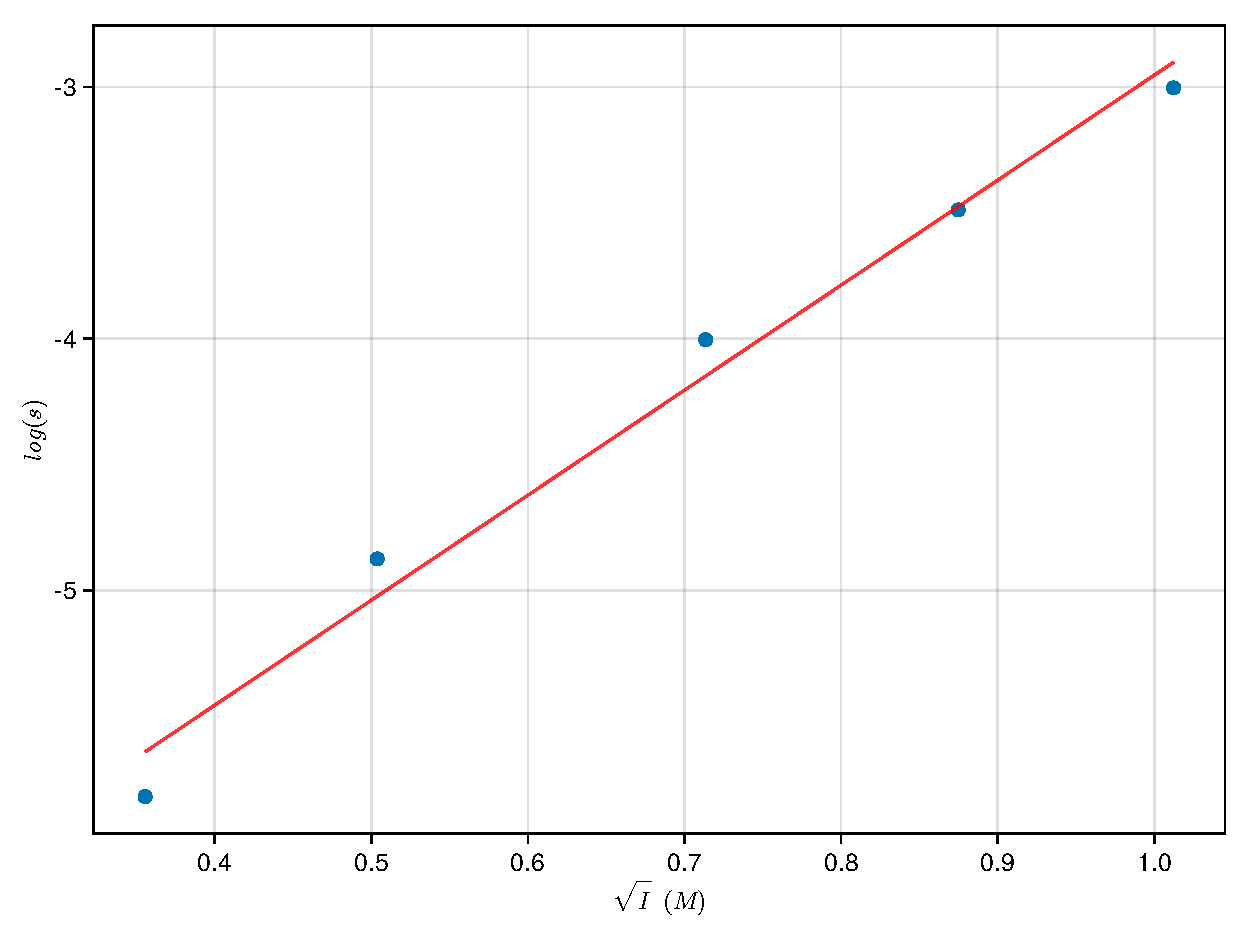
\includegraphics[width=\textwidth]{figures/regression.pdf}
    \caption{\(log(s)\) as a function of \(\sqrt{I}\)}
    \label{fig:regression}
\end{figure}


A static export of the notebook containing all analysis and figures is availible at \url{https://adammenne.github.io/chemistry_254/practical_2/plots.html}.\\ With full source code availble at \url{https://github.com/AdamMenne/chemistry_254/tree/master/practical_2}

\section{Discussion}

The fit on the linear regression has a percent error of 0.2307 and  0.3152 for the intercept and slope respectively. This indicates, atleast approximately, a linear relationship, as is expected from \(log(s) = log(s_0) + Kz_+ z_- \sqrt{I}\). See \cref{fig:regression}

Beyond this it is difficult to assess the accuracy of our data, without comparing to known values.

\newpage

\begin{appendices}

\section{Additional tasks}

\begin{enumerate}
    \item 0.002
    \item 0.006
\end{enumerate}



\section{Flow Diagram}

\begin{enumerate}
    \item Pipette 5 \(cm^3\) of one of five solutions of different concentration into a Erlenmeyer flask.
    \item Add \(\pm 10 cm^3\) of \(1M\) HCl and \(\pm 10 cm^3\) of \(10\%\) KI into the flask.
    \item Wait for three minutes, and titrate using thiosulphate solution, adding starch indicator towards the endpoint.
    \item Repeat twice.
    \item Repeat 1 through 4 for the other four solutions
\end{enumerate}

\section{MSDS}

\subsection*{Potassium nitrate}

\begin{itemize}
    \item Oxidising, harmful
    \item[-] may cause eye damage and respiratory irritation
    \item[-] keep away from ignition sources and combustable material 
    \item[-] keep away from skin and eyes 
\end{itemize}

\subsection*{Silver bromate}

\begin{itemize}
    \item Oxidising, harmful
    \item[-] may cause skin burns, eye damage and respiratory inflammation 
    \item[-] keep away from ignition sources and combustable material 
    \item[-] if in contact with skin or eyes wash for several minutes  
\end{itemize}

\subsection*{Hydrochloric acid}

\begin{itemize}
    \item Harmful, corrisive
    \item[-] may cause skin burns, eye damage and respiratory irritation, do not inhale
    \item[-] if in contact with skin or eyes wash for several minutes  
\end{itemize}

\subsection*{Potassium iodide}

\begin{itemize}
    \item Harmful
    \item[-] may cause skin and eye irritation
    \item[-] if in contact with skin or eyes wash for several minutes 
\end{itemize}
    
\end{appendices}

\end{document}